\documentclass[12pt,a4paper]{article}

%\usepackage[ngerman]{babel}
\usepackage[utf8x]{inputenc}
\usepackage[T1]{fontenc}

%\usepackage[hyphens]{url}
\usepackage{float}
\usepackage[breaklinks]{hyperref}
\usepackage[hyphenbreaks]{breakurl}
\usepackage{breakurl}
\usepackage{placeins}
\usepackage{wrapfig}
\usepackage{rotating}
\usepackage{titlesec}
\usepackage{hvfloat}
\usepackage{lipsum}
\usepackage{palatino}
\usepackage{a4wide}
\usepackage{multicol}
\usepackage{float}
\usepackage{graphicx}
\usepackage{amsfonts}
\usepackage{amsmath}
\usepackage{mathtools}
\usepackage{amsthm}
\usepackage{amssymb}
\usepackage{array}
\usepackage{listings}
\usepackage{colortbl}
\usepackage{endnotes}
\usepackage{inconsolata}
\usepackage{epstopdf}
\usepackage{blindtext}
\usepackage{color}
\usepackage{pdflscape}
\usepackage{capt-of}
\usepackage{sidecap}
\usepackage[usenames,dvipsnames]{xcolor}
\usepackage{tikzsymbols}
\usepackage{phaistos}
\usepackage{bbding}
\usepackage[francais,english,german]{babel}
%\usepackage{fontawesome}
%\usepackage[small,compact]{titlesec}
\usepackage{tikz}
%\usetikzlibrary{arrows,automata}

\definecolor{light-gray}{gray}{0.95}

\usepackage{booktabs}                   %gives \toprule, \midrule and \bottomrule for professional looking tables
\usepackage{fixltx2e}                   %fixltx2e adds \textsubscript{}, textsubscript should already be there
\usepackage{threeparttable}             %Provides notes in tables (in addition to the caption)
\usepackage{tabularx}                   %Defines column type X for tables with auto linebreaks. For REALLY big tables use one of the more specialized packages
\usepackage{caption}
%\usepackage{subcaption}
%\captionsetup{margin=0.8cm,aboveskip=8mm,labelfont=bf,labelformat=simple,labelsep=period,textfont=small}
% \setcounter{tocdepth}{2}        %Two should be default anyway
% \setlength{\parskip}{1ex plus 0.5ex minus 0.5ex}        %Space of a paragraph, note the variability, gives latex more room for optimization
\titlespacing{\section}{0pt}{20pt}{16pt}
\titlespacing{\subsection}{0pt}{20pt}{16pt}
\titlespacing{\subsubsection}{0pt}{20pt}{16pt}
\setlength{\parindent}{0pt}       %Basically a whole lot of \noindents before every paragraph ;)
\usepackage{nicefrac}                   %fraction style (a/b) use with \nicefrac{}{}
% \setlength{\headheight}{15pt}
% \usepackage{emptypage}          %Empty pages are really empty, no header or anything

\lstset{
 language=AWK,                % choose the language of the code
 basicstyle=\footnotesize,       % the size of the fonts that are used for the code
 numbers=left,                   % where to put the line-numbers
 numberstyle=\footnotesize,      % the size of the fonts that are used for the line-numbers
 stepnumber=1,                   % the step between two line-numbers. If it is 1 each line will be numbered
 numbersep=10pt,                  % how far the line-numbers are from the code
 showspaces=false,               % show spaces adding particular underscores
 showtabs=false,                 % show tabs within strings adding particular underscores
 frame=single,   		% adds a frame around the code
 tabsize=4,  		% sets default tabsize to 2 spaces
 captionpos=t,   		% sets the caption-position to bottom
 breaklines=true,    	% sets automatic line breaking
 breakatwhitespace=false,    % sets if automatic breaks should only happen at whitespace
 showstringspaces=false,
 mathescape=false,		%allo entering math environment
 backgroundcolor=\color{light-gray},
 morekeywords={init, par, foreach, return, min, allocate, abs, delete, is_member, insert},            % if you want to add more keywords to the set
 keywordstyle=\color{blue},          % keyword style
 commentstyle=\color{OliveGreen},       % comment style
 stringstyle=\color{orange}
}

\hypersetup{
    bookmarks=true,         % show bookmarks bar?
    unicode=true,          % non-Latin characters in Acrobat’s bookmarks
    pdftoolbar=true,        % show Acrobat’s toolbar?
    pdfmenubar=true,        % show Acrobat’s menu?
    pdffitwindow=false,     % window fit to page when opened
    pdfstartview={Fit},    % fits the width of the page to the window
    pdftitle={Homework 2:  Modélisation des écosystèmes aquatiques - Nicolas Piret et Yann Sp\"ori},    % title
    pdfauthor={Nicolas Piret et Yann Sp\"ori},     % author
    %pdfsubject={Subject},   % subject of the document
    %pdfcreator={Creator},   % creator of the document
    %pdfproducer={Producer}, % producer of the document
    %pdfkeywords={keywords}, % list of keywords
    pdfnewwindow=true,      % links in new window
    colorlinks=false,       % false: boxed links; true: colored links
    linkcolor=red,          % color of internal links
    citecolor=green,        % color of links to bibliography
    filecolor=magenta,      % color of file links
    urlcolor=cyan           % color of external links
}

\newcommand{\citeme}[1]{\Large\textsuperscript{\textbf{\textcolor{Blue}{cite me!}(#1)}}\normalsize}
\newcommand{\todo}{\textbf{\textcolor{red}{ TODO! }}}
\newcommand{\refer}[1]{\ref{#1}~(page~\pageref{#1})}
\newcommand{\al}[0]{$\alpha$}
\newcommand{\alimp}[0]{$\alpha$\,IMP\ }
\newcommand{\alimps}[0]{$\alpha$\,IMPs\ }   %These are not nice, could have used sth like \al-IMPs or {\alimp}s
\newcommand{\be}[0]{$\beta$}
\newcommand{\beimp}[0]{$\beta$\,IMP\ }
\newcommand{\beimps}[0]{$\beta$\,IMPs\ }
\newcommand{\supp}[0]{Supplementary Material\ }
\newcommand{\angs}[0]{\,\AA}
\newcommand{\method}[1]{\textbf{#1}}
\newcommand{\ie}[0]{\textit{i.e.\ }}
\newcommand{\eg}[0]{e.g.\ }
\newcommand{\cf}[0]{cf.\ }
\newcommand{\chap}[0]{cp.\ }
\newcommand{\dbid}[1]{{\fontfamily{phv}\selectfont\footnotesize\lowercase{#1}}}   
\newcommand{\figintro}[1]{\textbf{#1}}
\newcommand\abs[1]{\left|#1\right|}
\newcommand{\highlight}[1]{%
  \colorbox{yellow!50}{$\displaystyle#1$}}
\newcommand{\highlightgreen}[1]{%
  \colorbox{green!50}{$\displaystyle#1$}}
\newcommand{\hr}[0]{
\par{
\noindent\makebox[\linewidth]{\rule{\textwidth}{1pt}}
}
}

\usepackage[sort&compress,comma,numbers]{natbib}

% table of contents
\renewcommand{\contentsname}{Table of contents}

% Bibliography
\usepackage[numbib,notlof,notlot,nottoc,section]{tocbibind}
\renewcommand\tocbibname{References}

\setcounter{secnumdepth}{4}

\titleformat{\paragraph}
{\normalfont\normalsize\bfseries}{\theparagraph}{1em}{}
\titlespacing*{\paragraph}
{0pt}{3.25ex plus 1ex minus .2ex}{1.5ex plus .2ex}

\usepackage{xcolor}
\definecolor{c0}{Hsb}{000,1.0,0.5}
\definecolor{c1}{Hsb}{024,1.0,0.5}
\definecolor{c2}{Hsb}{048,1.0,0.5}
\definecolor{c3}{Hsb}{072,1.0,0.5}
\definecolor{c4}{Hsb}{096,1.0,0.5}
\definecolor{c5}{Hsb}{120,1.0,0.5} 
\definecolor{c6}{Hsb}{144,1.0,0.5}
\definecolor{c7}{Hsb}{168,1.0,0.5}
\definecolor{c8}{Hsb}{192,1.0,0.5}
\definecolor{c9}{Hsb}{216,1.0,0.5}
\definecolor{cA}{Hsb}{240,1.0,0.5}
\definecolor{cB}{Hsb}{264,1.0,0.5}
\definecolor{cC}{Hsb}{288,1.0,0.5}
\definecolor{cD}{Hsb}{312,1.0,0.5}
\definecolor{cE}{Hsb}{336,1.0,0.5}
\definecolor{cF}{Hsb}{360,1.0,0.5}

\titleformat{\section}[block]
  {\fontsize{12}{15}\bfseries\sffamily}%\filcenter}
  {\thesection}
  {1em}
  {\MakeUppercase}
\titleformat{\subsection}[block]
  {\fontsize{12}{15}\bfseries\sffamily}
  {\thesubsection}
  {1em}
  {}
\titleformat{\subsubsection}[block]
  {\fontsize{12}{15}\bfseries\sffamily}
  {\thesubsubsection}
  {1em}
  {}

\begin{document}

% TITLE PAGE
{
\selectlanguage{francais}
\pagenumbering{gobble}
\raggedleft

\includegraphics[width=0.15\textwidth]{ulbnorm.jpg}
\par\vspace{-1.8cm}
\centering
{\scshape\LARGE Université libre de Bruxelles \par}
\vspace{2.4cm}
{\Huge\bfseries BING-F525 - Modélisation des écosystèmes aquatiques\par}
\vspace{1.2cm}
{\Large\bfseries Travaux Pratiques\par}
\vspace{1.0cm}
{\LARGE\bfseries Croissance du zooplancton\par}
\vspace{1.5cm}
%\vfill
{\Large\itshape Nicolas Piret\\Master en bioingénieur : sciences et technologies de l'environnement\par}
\vspace{0.5cm}
{\Large\itshape Yann Spöri\\Master en bioinformatique et modélisation\par}
\vfill
course donne par\par
Nathalie Gypens%\textsc{Brown}
\vfill
% Bottom of the page
\begin{center}{\large \today}\end{center}
}
\newpage
\pagenumbering{arabic}
% END TITLE PAGE

% add table of contents
\selectlanguage{francais} % Dit a babel que le rapport est écrit en français 
\tableofcontents
\newpage

% introduction
\section{Introduction}

\FloatBarrier
% la première partie
\section{Module de croissance du zooplancton}

\subsection{Description du module}
\par{
Dans les travaux pratiques précédents on a analysé la croissance du phytoplancton en fonction des
nutriments disponibles. Dans les modèles actuels nous sommes moins intéressés par l'approvisionnement
alimentaire du phytoplancton. Nous avons plutôt procédé par enquêter l'interaction du phytoplancton avec
un prédateur naturel de cette espèce, le zooplancton. En conséquence le modèle mathèmatique a été simplifié
de manière à ce qu'on considère maintenant une offre des nutriments infiniment grand pour le
phytoplancton\footnote{En d'autres termes, la croissance du phytoplancton n'est plus limitée par les
nutriments}.
\par{
Pour mieux interpréter les simulations du modèle mathématique nous avons émis l'hypothèse que la mortalité
du phytoplancton est uniquement due au broutage du zooplancton. La mortalité du phytoplancton par d'autres
prédateurs, toxines environnementales, lyse cellulaire etc. n'est pas représentée par le modèle.
Nous supposons donc que l'influence de ces causes de mortalité peut être négligée par rapport à l'influence
de la mortalité de phytoplancton due au broutage du zooplancton.
}
\par{
En résumé, nous obtenons le modèle conceptuel effectué dans la figure~\ref{fig:partie1DiagConcept}
et les équations suivantes:
}

\begin{equation}
  {{d[DA]}\over{dt}} =
  \mu_{DA} [DA] - graz_{MSZ} [MSZ]
  \label{eq:partie1DiffEq1}
\end{equation}
\begin{equation}
  {{d[MSZ]}\over{dt}} =
  \left (
    (1- eges_{MSZ}) graz_{MSZ} Y_{MSZ} - mm_{MSZ}
  \right ) [MSZ]
  \label{eq:partie1DiffEq2}
\end{equation}

\par{
Dans la première partie des travaux pratiques, l'intérêt principal est de comparer l'impacte de la
fonctions de broutage. Pour les analyses, les fonctions de broutage suivantes ont été considérées:
}

\begin{equation}
  graz_{MSZ} = g_{MSZ} \max(T) {{[DA]}\over{kg_{MSZ}+[DA]}}
  \label{eq:partie1GrazMic}
\end{equation}
\begin{equation}
  graz_{MSZ} = g_{MSZ} \max(T) {{[DA]-[DA_0]}\over{kg_{MSZ}+([DA]-[DA_0])}}
  \label{eq:partie1GrazMicSeul}
\end{equation}
\begin{equation}
  graz_{MSZ} = g_{MSZ} \max(T) {{[DA]^2}\over{kg_{MSZ}^2+[DA]^2}}
  \label{eq:partie1GrazHol}
\end{equation}

\begin{figure}[h!]
  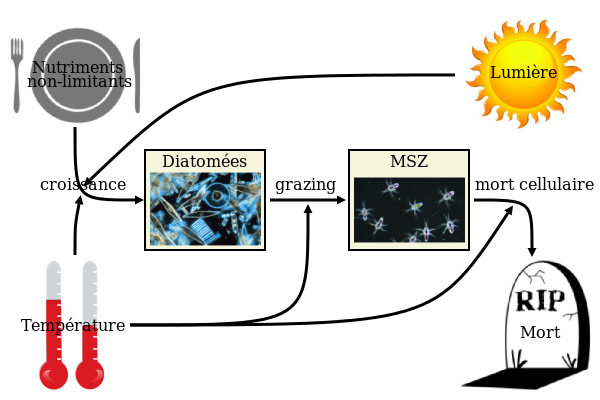
\includegraphics[width=\textwidth]{partie1/diagrammeConceptuel.png}
  \caption{Le modèle conceptuel du système étudié dans le quatrième cours. La croissance du phytoplancton
n'est plus limitée par les nutriments disponibles. Cependant, la croissance est toujours limitée par la
disponibilité de la lumière et de la température. Dans les formules, l'influence de ces deux impacts
environnementals est cachée dans le terme $\mu_{DA}$. Une partie du phytoplancton existant est consommer
par le mésozooplancton (=MSZ). Cette partie est représentée par les fonctions de broutage
différentes fois la concentration du mésozooplancton ($graz_{MSZ}[MSZ]$). Dans le système modèlise
le mésozooplancton n'a pas des prédateurs naturels. Donc, la mort cellulaire naturelle du zooplancton ne peut
plus être négligée (dans les formules c'est le terme $mm_{MSZ}$ qui décrit cette l'influence).
}
  \label{fig:partie1DiagConcept}
\end{figure}

\par{
Pour peut mieux comprendre les équations du modèle, la grille~\ref{tab:partie1signifParam} peut également
être intéressante. Elle donne un aperçu de la signification etc. de chaque terme dans les équations.
}
\par{
Nous voulons encore pointer que les $T_{opt}$ et $d_{opt}$ ont les mêmes valeurs pour les diatomées et le
mésozooplancton simulé. On a donc considerer que les deux espèces sont limitées par la tempèrature
de la même façon.
}

\begin{table}[h!]
\begin{center}
\begin{tabular}{ | c | c | c | c | c | }
\hline
Terme & Signification & Type & Valeur & Unité \\
\hline
$[DA]$ & \pbox{4cm}{Concentration du carbon des diatomées} & Variable d'état & $5$ & ${{mmol C}\over{m^{-3}}}$ \\
$[MSZ]$ & \pbox{4cm}{Concentration du carbon du mésozooplancton}  & Variable d'état & $1$ & ${{mmol C}\over{m^{-3}}}$ \\
$\mu_{DA}$ & \pbox{4cm}{Taux de croissance des diatomées} & \pbox{3cm}{Fonction $\mu_{max}max(T)llum$} & \pbox{4cm}{Dépend de la disponibilité de la lumière (en fonction du $[DA]$) et de la tempèrature} & $Jour^{-1}$ \\
$graz_{MSZ}$ & \pbox{4cm}{Fonction de grazing} & Fonction & \pbox{4cm}{Dépend de la tempèrature et de $[DA]$} & $Jour^{-1}$ \\
$eges_{MSZ}$ & \pbox{4cm}{Taux d'egestion du mésozooplancton} & Paramètre & $0.1$ & $-$ \\
$Y_{MSZ}$ & \pbox{4cm}{Efficience de croissance du mésozooplancton} & Paramètre & $0.25$ & $-$ \\
$mm_{MSZ}$ & \pbox{4cm}{Taux de mortalité du mésozooplancton} & Paramètre & $0.05$ & $Jour^{-1}$ \\
$g_{MSZ}$ & \pbox{4cm}{Taux de grazing maximal} & Paramètre & $1.2$ & $Jour^{-1}$ \\
$max(T)$ & \pbox{4cm}{Fonction de la limitation de la tempèrature} & \pbox{3cm}{Fonction\\(bell-shaped)} & \pbox{4cm}{Dépend de $T, T_{opt}$ et $d_{opt}$} & $-$ \\
$kg_{MSZ}$ & \pbox{4cm}{Constante de grazing} & Paramètre & $10$ & ${{mmol C}\over{m^{-3}}}$ \\
$[DA_0]$ & \pbox{4cm}{Concentration minimale avant le mésozooplancton commencent de consummer les diatomées} & Paramètre & $5$ & ${{mmol C}\over{m^{-3}}}$ \\
$\mu_{max}$ & \pbox{4cm}{Taux de croissance maximal des diatomées} & Paramètre & $1.2$ & $Jour^{-1}$ \\
$T_{opt}$ & \pbox{4cm}{Température optimale (pour les diatomées et du mésozooplancton)} & Paramètre & $16.3$ & $^{\circ}C$ \\
$d_{opt}$ & \pbox{4cm}{Delta T (pour les diatomées et du mésozooplancton)} & Paramètre & $13.7$ & $^{\circ}C$ \\
$T$ & \pbox{4cm}{Température simulée} & Paramètre & $10.0$ & $^{\circ}C$ \\
$llum$ & \pbox{4cm}{Limitation par la lumière} & \pbox{3cm}{Fonction\\$1-e^{-\alpha PAR_Z / \mu_{max}}$} & \pbox{4cm}{Dépend de la lumière disponible, ...} & $-$ \\
\end{tabular}
\end{center}
\end{table}
\clearpage
\begin{table}[h!]
\begin{center}
\begin{tabular}{ | c | c | c | c | c | }
$\alpha$ & \pbox{4cm}{L'efficacité des chloroplastes des diatomées} & Paramètre & $0.02$ & ${mol^{-1}*m^2*sec}\over{quanta * jour}$ \\
$PAR_Z$ & \pbox{4cm}{Lumière disponible par mol chlorophylle} & \pbox{3cm}{Fonction\\$PAR_0*e^{-k_e*z}$} & \pbox{4cm}{Dépend de la latitude, les solides en suspension, ...} & ${mol*quanta}\over{m^2*sec}$ \\
$PAR_0$ & \pbox{4cm}{Lumière solaire incidente} & Paramètre & $23.0$ & ${quanta}\over{m^2*sec}$ \\
$k_e$ & \pbox{4cm}{Coefficient d'extinction verticale de la lumière} & \pbox{3cm}{Fonction\\$0.35+0.02{{1}\over{2}}[DA]$} & \pbox{4cm}{Dépend des solides en suspension, ...} & $^{mol}/_m$ \\
$z$ & \pbox{4cm}{Profondeur de l'habitat} & Paramètre & $1.0$ & $m$ \\
\hline
\end{tabular}
\end{center}
  \caption{Signification, type, valeur et unité de chaque terme/paramètre dans les
équations~\ref{eq:partie1DiffEq1},~\ref{eq:partie1DiffEq2},~\ref{eq:partie1GrazMic},~\ref{eq:partie1GrazMicSeul} et~\ref{eq:partie1GrazHol}.}
  \label{tab:partie1signifParam}
\end{table}
\FloatBarrier

\subsection{Analyse mathèmatique}

\par{
La grille~\ref{tab:partie1etatsStat} donne un aperçu des états stationnaires du système
pour les fonctions de broutage differents. Les constantes supplémentaires utilisées
dans la grille sont définies comme suit:
}
\[
m = mm_{MSZ_{MAX_0}} e ^{- \left ( {{t-t_{opt}}\over{d_{opt}}} \right )}
\]
\[
k = kg_{MSZ}
\]
\[
c = \left ( 1 - eges_{MSZ} \right ) y_{MSZ}
g_{MSZ_{MAX_0}} e ^{- \left ( {{t-t_{opt}}\over{d_{opt}}} \right )}
\]
\[
f = g_{MSZ_{MAX_0}} e ^{- \left ( {{t-t_{opt}}\over{d_{opt}}} \right )}
\]

\begin{table}[h!]
\begin{center}
\begin{tabular}{ | c | c c | }
\hline
fct. de broutage & $[DA]$ & $[MSZ]$ \\
\hline
MIC, MIC\_Seul, HOL & 0 & 0 \\
MIC & $k * {{m}\over{c-m}}$ & ${{\mu_{DA} k \left ( 1 + {{m}\over{c-m}} \right )}\over{f}}$ \\
MIC\_Seuil & ${{m/c*k-m/c[DA_0]+[DA_0]}\over{1-m/c}}$ & ${\mu_{DA} * [DA] * (k + [DA] - [DA_0])}\over{f *([DA] - [DA_0])}$ \\
HOL & $k*\sqrt{{{m}\over{c-m}}}$ & ${{\mu_{DA}k \left ( 1 + {m}\over{c-m} \right )}\over{f \sqrt{{m}\over{c-m}}}}$ \\
\hline
\end{tabular}
\end{center}
  \caption{Les états stationnaires du système pour les fonctions de broutage differents. Les
constantes supplémentaires utilisées ont était définies dans le texte précédent. Les formules sont en accord
avec les simulations informatiques décrites ci-dessous.
}
  \label{tab:partie1etatsStat}
\end{table}
\FloatBarrier

\subsection{Simulation de référence}

\begin{figure}[h!]
  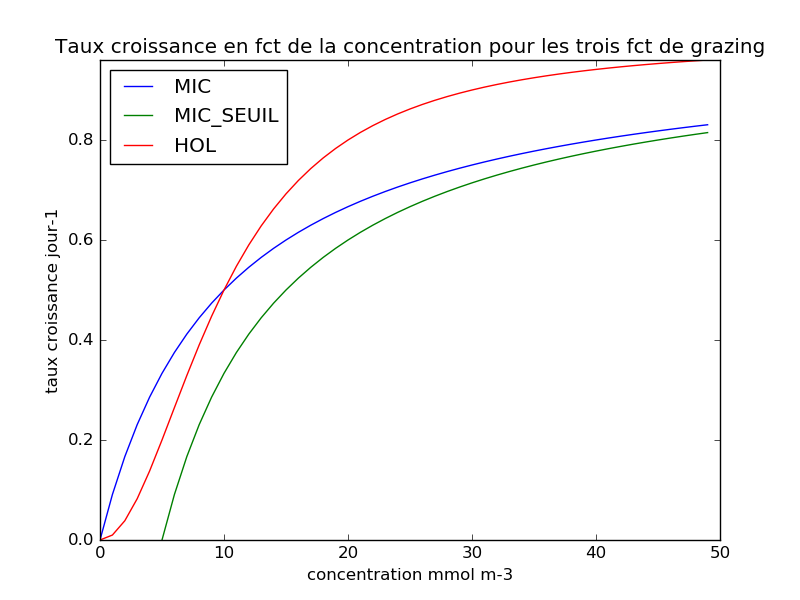
\includegraphics[width=\textwidth]{partie1/grazingFct.png}
  \caption{
La courbe de les trois fonctions~\ref{eq:partie1GrazMic} (MIC),~\ref{eq:partie1GrazMicSeul} (MIC\_SEUIL)
et~\ref{eq:partie1GrazHol} (HOL) en fonction de la concentration $[DA]$.
}
  \label{fig:partie1grazingFcts}
\end{figure}

\begin{figure}[h!]
  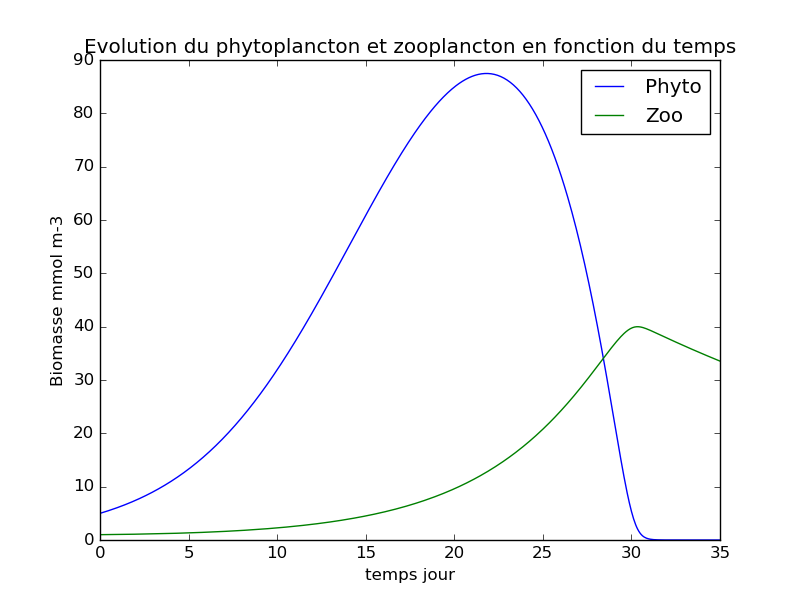
\includegraphics[width=0.5\textwidth]{partie1/refMic35.png}\hfill
  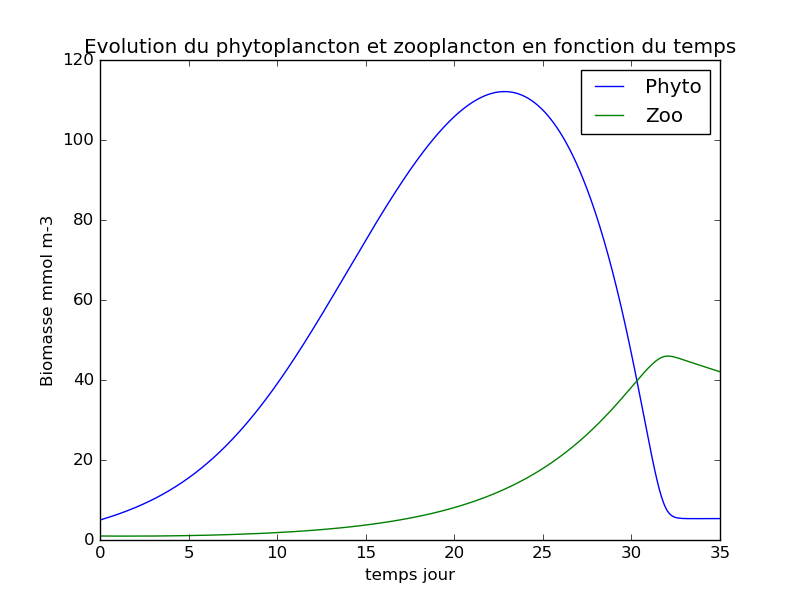
\includegraphics[width=0.5\textwidth]{partie1/refMicSeul35.png}\\
  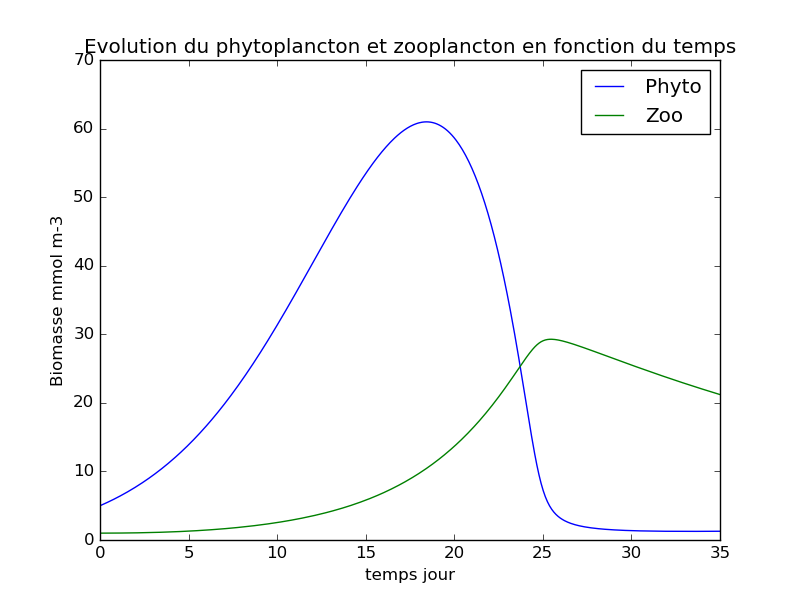
\includegraphics[width=0.5\textwidth]{partie1/refHol35.png}\hfill
  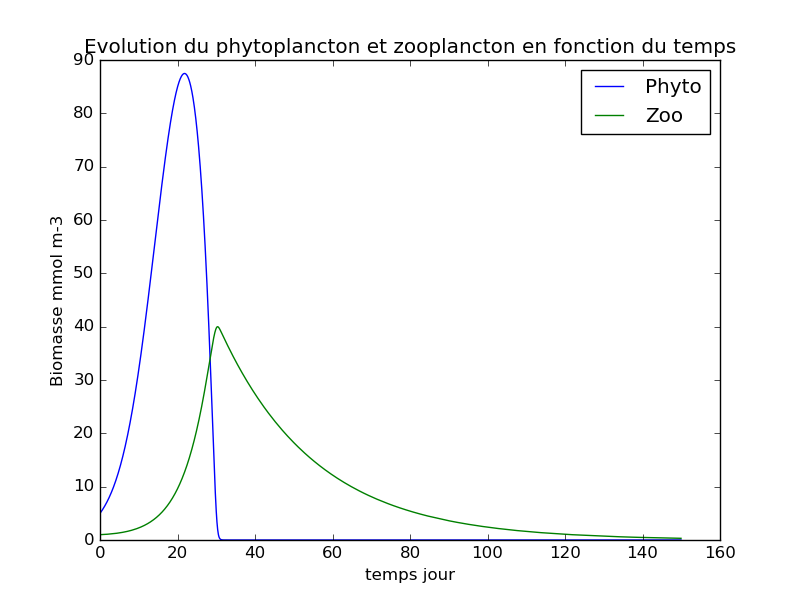
\includegraphics[width=0.5\textwidth]{partie1/refMic150.png}\\
  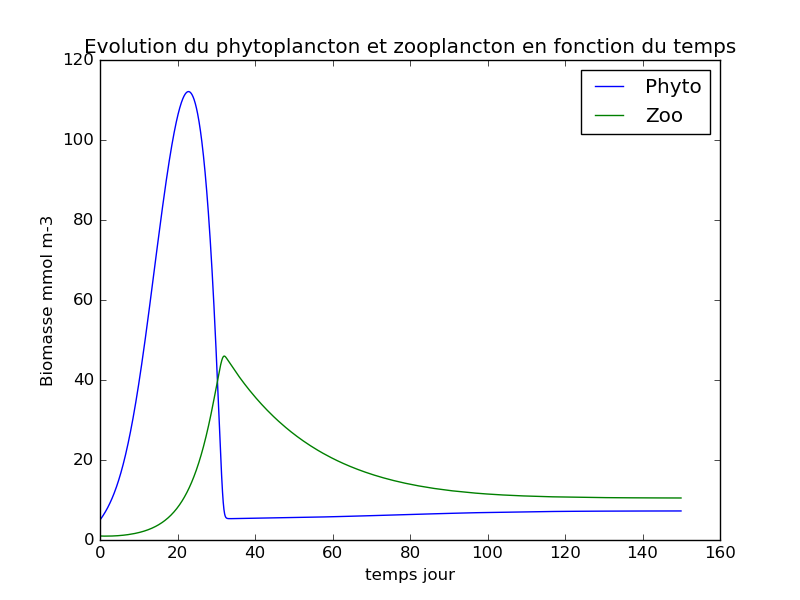
\includegraphics[width=0.5\textwidth]{partie1/refMicSeul150.png}\hfill
  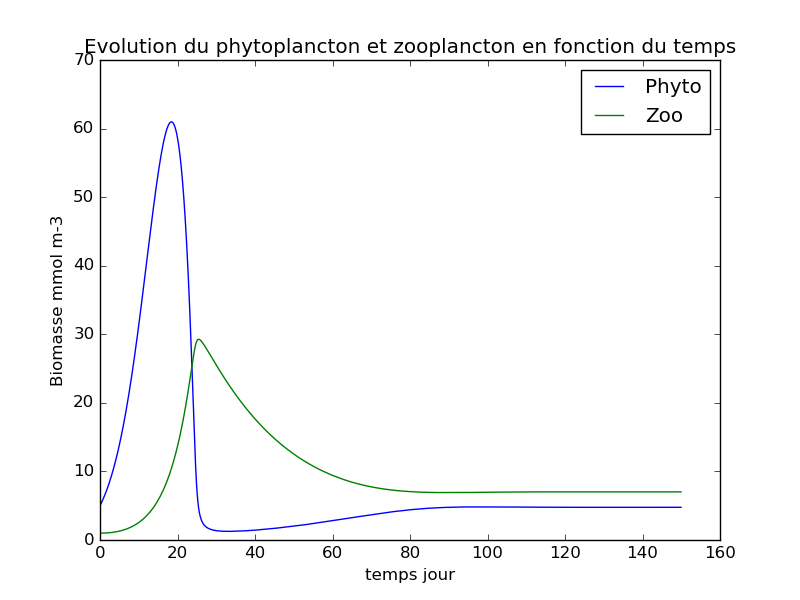
\includegraphics[width=0.5\textwidth]{partie1/refHol150.png}
  \caption{\todo}
  \label{fig:partie1RefSimulations}
\end{figure}

\subsection{Simulation de test 1}


\FloatBarrier
% la deuxième partie
%\section{Module de croissance du zooplancton}

\subsection{Description du module}
\par{
Dans les travaux pratiques précédents on a analysé la croissance du phytoplancton en fonction des
nutriments disponibles. Dans les modèles actuels nous sommes moins intéressés par l'approvisionnement
alimentaire du phytoplancton. Nous avons plutôt procédé par enquêter l'interaction du phytoplancton avec
un prédateur naturel de cette espèce, le zooplancton. En conséquence le modèle mathèmatique a été simplifié
de manière à ce qu'on considère maintenant une offre des nutriments infiniment grand pour le
phytoplancton\footnote{En d'autres termes, la croissance du phytoplancton n'est plus limitée par les
nutriments}.
\par{
Pour mieux interpréter les simulations du modèle mathématique nous avons émis l'hypothèse que la mortalité
du phytoplancton est uniquement due au broutage du zooplancton. La mortalité du phytoplancton par d'autres
prédateurs, toxines environnementales, lyse cellulaire etc. n'est pas représentée par le modèle.
Nous supposons donc que l'influence de ces causes de mortalité peut être négligée par rapport à l'influence
de la mortalité de phytoplancton due au broutage du zooplancton.
}
\par{
En résumé, nous obtenons le modèle conceptuel effectué dans la figure~\ref{fig:partie1DiagConcept}
et les équations suivantes:
}

\begin{equation}
  {{d[DA]}\over{dt}} =
  \mu_{DA} [DA] - graz_{MSZ} [MSZ]
  \label{eq:partie1DiffEq1}
\end{equation}
\begin{equation}
  {{d[MSZ]}\over{dt}} =
  \left (
    (1- eges_{MSZ}) graz_{MSZ} Y_{MSZ} - mm_{MSZ}
  \right ) [MSZ]
  \label{eq:partie1DiffEq2}
\end{equation}

\par{
Dans la première partie des travaux pratiques, l'intérêt principal est de comparer l'impacte de la
fonctions de broutage. Pour les analyses, les fonctions de broutage suivantes ont été considérées:
}

\begin{equation}
  graz_{MSZ} = g_{MSZ} \max(T) {{[DA]}\over{kg_{MSZ}+[DA]}}
  \label{eq:partie1GrazMic}
\end{equation}
\begin{equation}
  graz_{MSZ} = g_{MSZ} \max(T) {{[DA]-[DA_0]}\over{kg_{MSZ}+([DA]-[DA_0])}}
  \label{eq:partie1GrazMicSeul}
\end{equation}
\begin{equation}
  graz_{MSZ} = g_{MSZ} \max(T) {{[DA]^2}\over{kg_{MSZ}^2+[DA]^2}}
  \label{eq:partie1GrazHol}
\end{equation}

\begin{figure}[h!]
  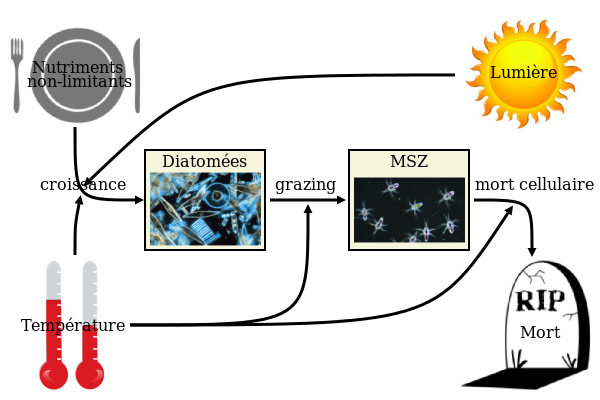
\includegraphics[width=\textwidth]{partie1/diagrammeConceptuel.png}
  \caption{Le modèle conceptuel du système étudié dans le quatrième cours. La croissance du phytoplancton
n'est plus limitée par les nutriments disponibles. Cependant, la croissance est toujours limitée par la
disponibilité de la lumière et de la température. Dans les formules, l'influence de ces deux impacts
environnementals est cachée dans le terme $\mu_{DA}$. Une partie du phytoplancton existant est consommer
par le mésozooplancton (=MSZ). Cette partie est représentée par les fonctions de broutage
différentes fois la concentration du mésozooplancton ($graz_{MSZ}[MSZ]$). Dans le système modèlise
le mésozooplancton n'a pas des prédateurs naturels. Donc, la mort cellulaire naturelle du zooplancton ne peut
plus être négligée (dans les formules c'est le terme $mm_{MSZ}$ qui décrit cette l'influence).
}
  \label{fig:partie1DiagConcept}
\end{figure}

\par{
Pour peut mieux comprendre les équations du modèle, la grille~\ref{tab:partie1signifParam} peut également
être intéressante. Elle donne un aperçu de la signification etc. de chaque terme dans les équations.
}
\par{
Nous voulons encore pointer que les $T_{opt}$ et $d_{opt}$ ont les mêmes valeurs pour les diatomées et le
mésozooplancton simulé. On a donc considerer que les deux espèces sont limitées par la tempèrature
de la même façon.
}

\begin{table}[h!]
\begin{center}
\begin{tabular}{ | c | c | c | c | c | }
\hline
Terme & Signification & Type & Valeur & Unité \\
\hline
$[DA]$ & \pbox{4cm}{Concentration du carbon des diatomées} & Variable d'état & $5$ & ${{mmol C}\over{m^{-3}}}$ \\
$[MSZ]$ & \pbox{4cm}{Concentration du carbon du mésozooplancton}  & Variable d'état & $1$ & ${{mmol C}\over{m^{-3}}}$ \\
$\mu_{DA}$ & \pbox{4cm}{Taux de croissance des diatomées} & \pbox{3cm}{Fonction $\mu_{max}max(T)llum$} & \pbox{4cm}{Dépend de la disponibilité de la lumière (en fonction du $[DA]$) et de la tempèrature} & $Jour^{-1}$ \\
$graz_{MSZ}$ & \pbox{4cm}{Fonction de grazing} & Fonction & \pbox{4cm}{Dépend de la tempèrature et de $[DA]$} & $Jour^{-1}$ \\
$eges_{MSZ}$ & \pbox{4cm}{Taux d'egestion du mésozooplancton} & Paramètre & $0.1$ & $-$ \\
$Y_{MSZ}$ & \pbox{4cm}{Efficience de croissance du mésozooplancton} & Paramètre & $0.25$ & $-$ \\
$mm_{MSZ}$ & \pbox{4cm}{Taux de mortalité du mésozooplancton} & Paramètre & $0.05$ & $Jour^{-1}$ \\
$g_{MSZ}$ & \pbox{4cm}{Taux de grazing maximal} & Paramètre & $1.2$ & $Jour^{-1}$ \\
$max(T)$ & \pbox{4cm}{Fonction de la limitation de la tempèrature} & \pbox{3cm}{Fonction\\(bell-shaped)} & \pbox{4cm}{Dépend de $T, T_{opt}$ et $d_{opt}$} & $-$ \\
$kg_{MSZ}$ & \pbox{4cm}{Constante de grazing} & Paramètre & $10$ & ${{mmol C}\over{m^{-3}}}$ \\
$[DA_0]$ & \pbox{4cm}{Concentration minimale avant le mésozooplancton commencent de consummer les diatomées} & Paramètre & $5$ & ${{mmol C}\over{m^{-3}}}$ \\
$\mu_{max}$ & \pbox{4cm}{Taux de croissance maximal des diatomées} & Paramètre & $1.2$ & $Jour^{-1}$ \\
$T_{opt}$ & \pbox{4cm}{Température optimale (pour les diatomées et du mésozooplancton)} & Paramètre & $16.3$ & $^{\circ}C$ \\
$d_{opt}$ & \pbox{4cm}{Delta T (pour les diatomées et du mésozooplancton)} & Paramètre & $13.7$ & $^{\circ}C$ \\
$T$ & \pbox{4cm}{Température simulée} & Paramètre & $10.0$ & $^{\circ}C$ \\
$llum$ & \pbox{4cm}{Limitation par la lumière} & \pbox{3cm}{Fonction\\$1-e^{-\alpha PAR_Z / \mu_{max}}$} & \pbox{4cm}{Dépend de la lumière disponible, ...} & $-$ \\
\end{tabular}
\end{center}
\end{table}
\clearpage
\begin{table}[h!]
\begin{center}
\begin{tabular}{ | c | c | c | c | c | }
$\alpha$ & \pbox{4cm}{L'efficacité des chloroplastes des diatomées} & Paramètre & $0.02$ & ${mol^{-1}*m^2*sec}\over{quanta * jour}$ \\
$PAR_Z$ & \pbox{4cm}{Lumière disponible par mol chlorophylle} & \pbox{3cm}{Fonction\\$PAR_0*e^{-k_e*z}$} & \pbox{4cm}{Dépend de la latitude, les solides en suspension, ...} & ${mol*quanta}\over{m^2*sec}$ \\
$PAR_0$ & \pbox{4cm}{Lumière solaire incidente} & Paramètre & $23.0$ & ${quanta}\over{m^2*sec}$ \\
$k_e$ & \pbox{4cm}{Coefficient d'extinction verticale de la lumière} & \pbox{3cm}{Fonction\\$0.35+0.02{{1}\over{2}}[DA]$} & \pbox{4cm}{Dépend des solides en suspension, ...} & $^{mol}/_m$ \\
$z$ & \pbox{4cm}{Profondeur de l'habitat} & Paramètre & $1.0$ & $m$ \\
\hline
\end{tabular}
\end{center}
  \caption{Signification, type, valeur et unité de chaque terme/paramètre dans les
équations~\ref{eq:partie1DiffEq1},~\ref{eq:partie1DiffEq2},~\ref{eq:partie1GrazMic},~\ref{eq:partie1GrazMicSeul} et~\ref{eq:partie1GrazHol}.}
  \label{tab:partie1signifParam}
\end{table}
\FloatBarrier

\subsection{Analyse mathèmatique}

\par{
La grille~\ref{tab:partie1etatsStat} donne un aperçu des états stationnaires du système
pour les fonctions de broutage differents. Les constantes supplémentaires utilisées
dans la grille sont définies comme suit:
}
\[
m = mm_{MSZ_{MAX_0}} e ^{- \left ( {{t-t_{opt}}\over{d_{opt}}} \right )}
\]
\[
k = kg_{MSZ}
\]
\[
c = \left ( 1 - eges_{MSZ} \right ) y_{MSZ}
g_{MSZ_{MAX_0}} e ^{- \left ( {{t-t_{opt}}\over{d_{opt}}} \right )}
\]
\[
f = g_{MSZ_{MAX_0}} e ^{- \left ( {{t-t_{opt}}\over{d_{opt}}} \right )}
\]

\begin{table}[h!]
\begin{center}
\begin{tabular}{ | c | c c | }
\hline
fct. de broutage & $[DA]$ & $[MSZ]$ \\
\hline
MIC, MIC\_Seul, HOL & 0 & 0 \\
MIC & $k * {{m}\over{c-m}}$ & ${{\mu_{DA} k \left ( 1 + {{m}\over{c-m}} \right )}\over{f}}$ \\
MIC\_Seuil & ${{m/c*k-m/c[DA_0]+[DA_0]}\over{1-m/c}}$ & ${\mu_{DA} * [DA] * (k + [DA] - [DA_0])}\over{f *([DA] - [DA_0])}$ \\
HOL & $k*\sqrt{{{m}\over{c-m}}}$ & ${{\mu_{DA}k \left ( 1 + {m}\over{c-m} \right )}\over{f \sqrt{{m}\over{c-m}}}}$ \\
\hline
\end{tabular}
\end{center}
  \caption{Les états stationnaires du système pour les fonctions de broutage differents. Les
constantes supplémentaires utilisées ont était définies dans le texte précédent. Les formules sont en accord
avec les simulations informatiques décrites ci-dessous.
}
  \label{tab:partie1etatsStat}
\end{table}
\FloatBarrier

\subsection{Simulation de référence}

\begin{figure}[h!]
  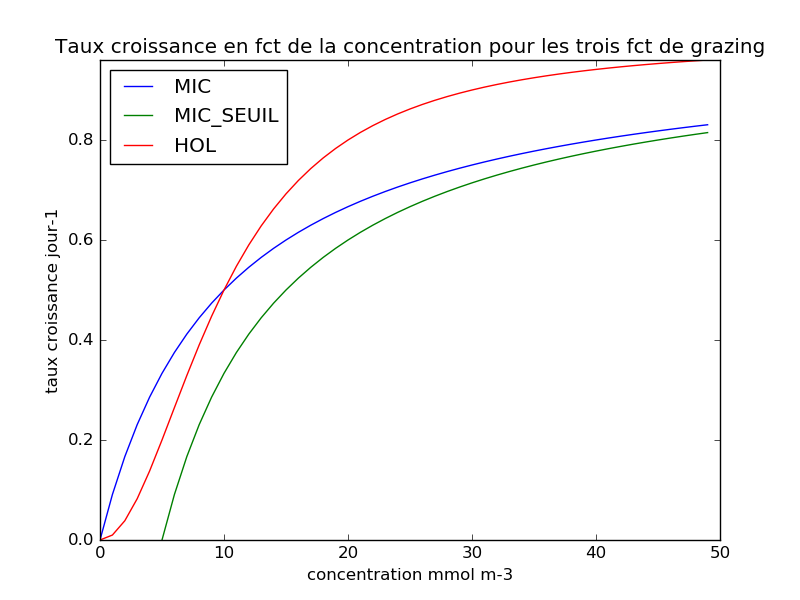
\includegraphics[width=\textwidth]{partie1/grazingFct.png}
  \caption{
La courbe de les trois fonctions~\ref{eq:partie1GrazMic} (MIC),~\ref{eq:partie1GrazMicSeul} (MIC\_SEUIL)
et~\ref{eq:partie1GrazHol} (HOL) en fonction de la concentration $[DA]$.
}
  \label{fig:partie1grazingFcts}
\end{figure}

\begin{figure}[h!]
  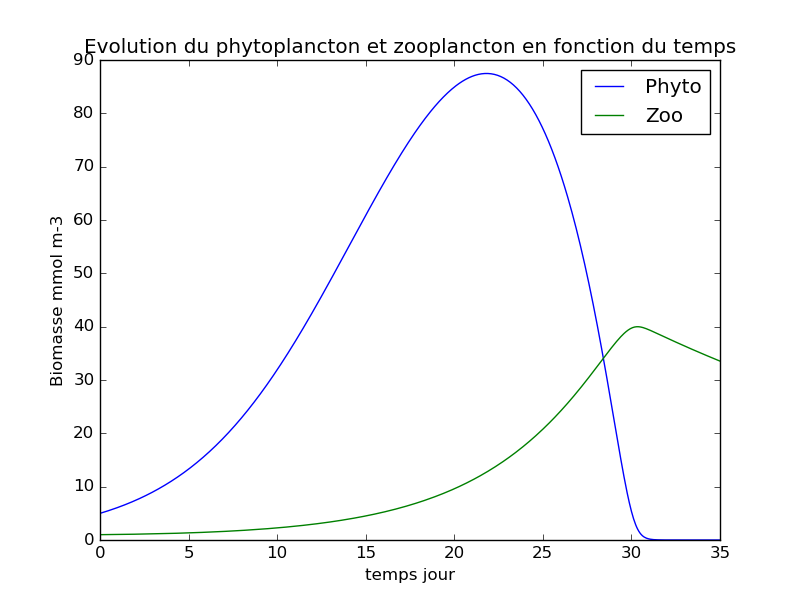
\includegraphics[width=0.5\textwidth]{partie1/refMic35.png}\hfill
  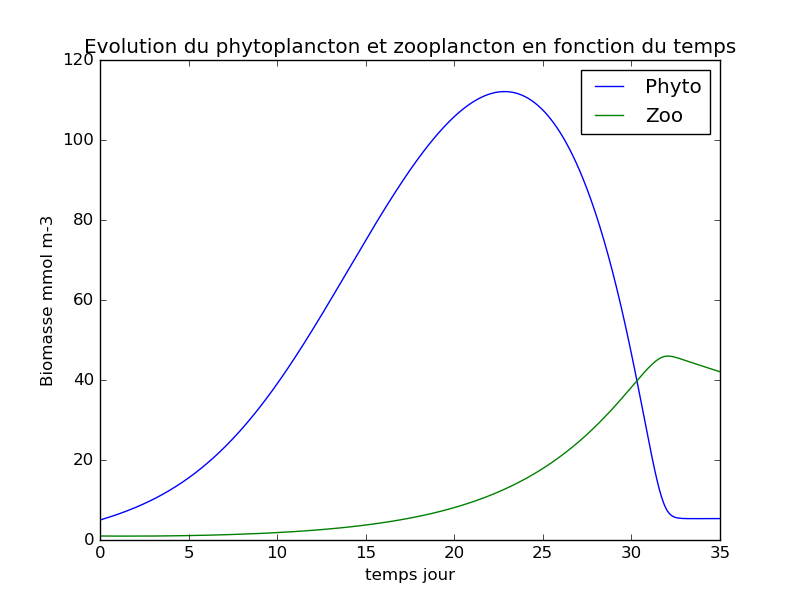
\includegraphics[width=0.5\textwidth]{partie1/refMicSeul35.png}\\
  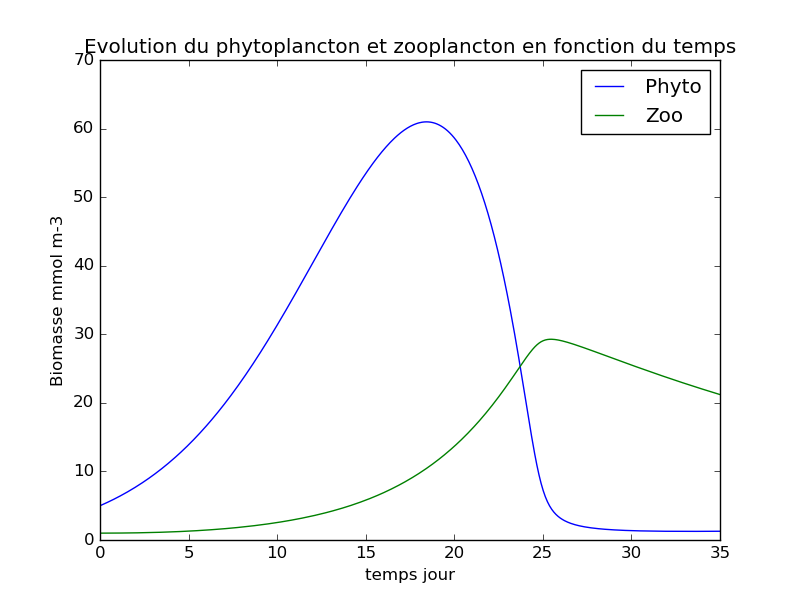
\includegraphics[width=0.5\textwidth]{partie1/refHol35.png}\hfill
  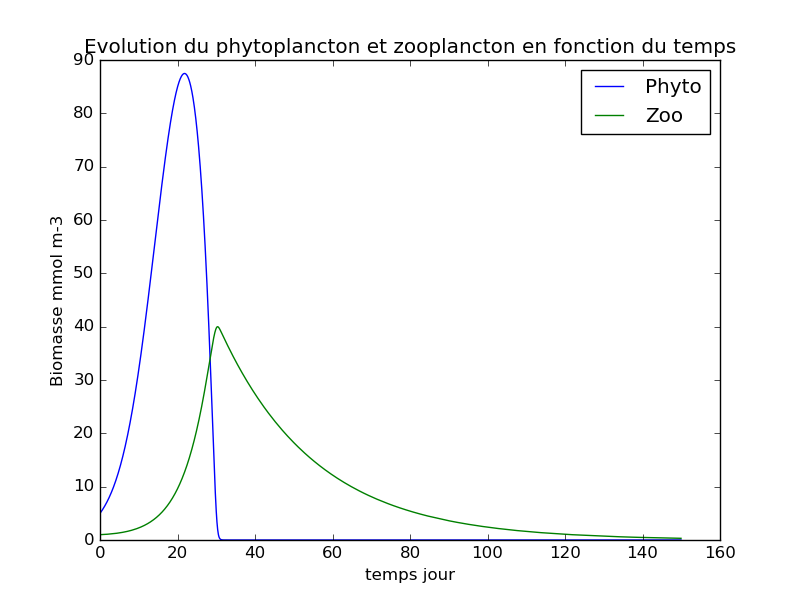
\includegraphics[width=0.5\textwidth]{partie1/refMic150.png}\\
  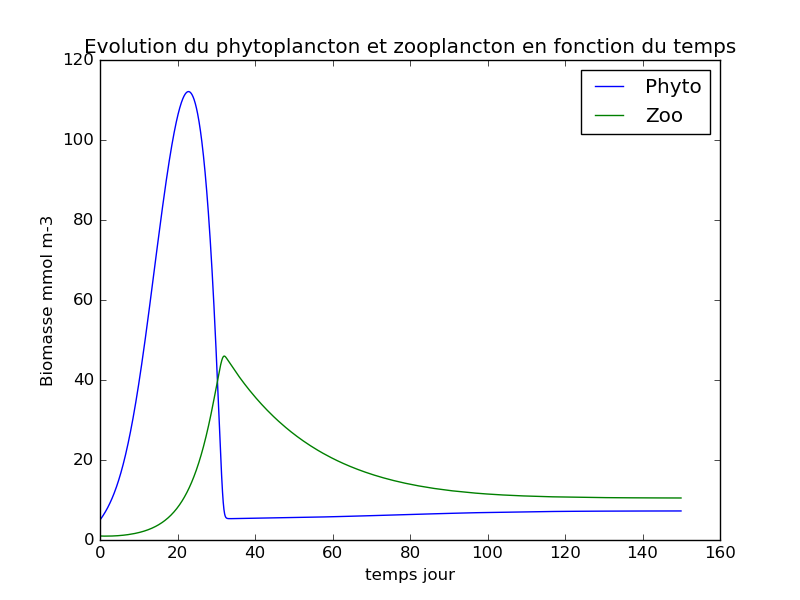
\includegraphics[width=0.5\textwidth]{partie1/refMicSeul150.png}\hfill
  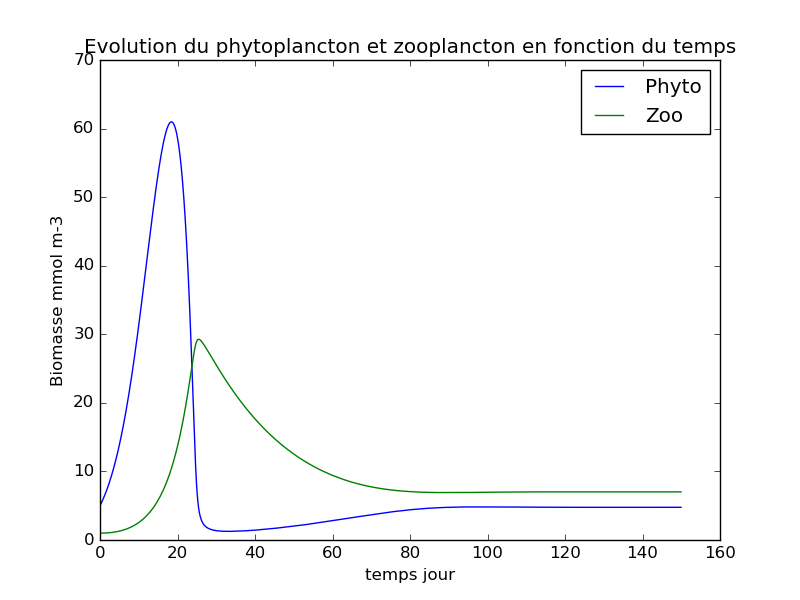
\includegraphics[width=0.5\textwidth]{partie1/refHol150.png}
  \caption{\todo}
  \label{fig:partie1RefSimulations}
\end{figure}

\subsection{Simulation de test 1}


%\FloatBarrier
% conclusion
\section{Conclusion}

\FloatBarrier

\end{document}
